% \section{Robust Reach-Avoid for Multi-Agent Systems}

\subsection{Solution Outline}
We summarize our approach for algorithmic solution of the posed problem in Alg.~\ref{alg:main}.

\begin{algorithm}[t]
	\caption{Multi-agent Controller Synthesis}
	\label{alg:main}
	\begin{enumerate}
		\item For every $i$, let $\Sigma_{\tau,\nom}^i = (X^i,x_\init^i,U^i,\set{0},f^i)$ be the respective \emph{nominal} control system that ignores the disturbances.
		Compute the product control system $\Sigma^\times_{\tau,\nom}$ of $\set{\Sigma^i_{\tau,\nom}}$. 
		%Let $\varepsilon\in \mathbb{R}^n_{>0}$ be a robustness margin. %a discussion on $\varepsilon$ follows subsequently.
		Use a scalable \emph{planner} to compute an open-loop controller $C^\times_{\nom}$ for $\Sigma^\times_{\tau,\nom}$ so that $C^\times_\nom\triangleright\Sigma_{\tau,\nom}^{\times}$ realizes  $\Phi_\varepsilon$.
		Let $T$ be the time horizon when $\Phi_\varepsilon$ has been fulfilled for the first time. \label{step:planning}
		\item Decompose $C^\times_\nom$ into \emph{local} open-loop controllers $\set{C^i_\nom}$ for the set of sampled-time abstractions $\set{\Sigma^i_{\tau,\nom}}$.
		The decomposition is straightforward since $C^\times_\nom$ is open-loop. Further, for every $i$, find the unique nominal open-loop trajectory $\rho^i=(x_{0,\nom}^i,\ldots,x_{T,\nom}^i)$ of length $T$ of $C^i_\nom\triangleright \Sigma_{\tau,\nom}^i$---unique, because there is no disturbance. \label{step:decompose}
		\item Let $\varepsilon^i\in \mathbb{R}^{n_i}_{>0}$ be the projection of $\varepsilon$ to the state dimensions of $\Sigma_{\tau}^i$.
		Use a \emph{guaranteed tracking} method to find a closed loop controller $C^i$ for $\Sigma_{\tau}^i$ so that $C^i\parallel \Sigma_\tau^i$ \emph{tracks} the nominal trajectory $\rho^i$, i.e., $C^i\parallel \Sigma_\tau^i$ satisfies the following specification:
		\begin{align}
			\label{eq:ltl_spec}
			\Phi_{\track}^i\coloneqq \ball_{\varepsilon^i}(x_{0,\nom}^i) \wedge \bigwedge_{k\in [1;T]} \bigcirc^t \ball_{\varepsilon^i}(x_{k,\nom}^i),
		\end{align}
		where %$\bigcirc$ denotes the next operator in LTL (\cite{baier2008principles}) and
		$\bigcirc^t$ represents the juxtaposition of $t$ consecutive ``$\bigcirc$'' operators.\label{step:tracking}
	\end{enumerate}
\end{algorithm}

It can be observed that if every  $C^i\parallel \Sigma_\tau^i$ can realize $\Phi_\track^i$, then because the simultaneous satisfaction of $\rho^i$-s for every $i$ implies satisfaction of $\Phi_\varepsilon$ by design, and because $\Phi_\varepsilon$ is an $\varepsilon$-robust version of $\Phi$, hence it follows that $\set{C^i}_{i\in [1;N]}\parallel \set{\Sigma_\tau^i}_{i\in [1;N]}$ will realize $\Phi$ under the worst-case disturbance. Next, we discuss our implementation for each of steps~\ref{step:planning} and \ref{step:tracking} in Alg.~\ref{alg:main}.

%We did not yet mention the role of the robustness margin $\varepsilon$.
%Essentially, $\varepsilon$ accounts for the possible tracking error of the ABCD-generated controller in Step~\ref{step:abcd} while tracking the nominal trajectory.
%Because ALTRO ignores the disturbances, hence a positive tracking error is inevitable.
%For this reason, if we choose $\varepsilon$ too small, then it will be more difficult for ABCD to find a controller against the worst case disturbances, and we might not be able to obtain a controller in Step~\ref{step:abcd} in the end.
%On the other hand, if we choose $\varepsilon$ too large, then it will be more difficult for ALTRO to find a nominal open-loop controller in the first place.
%So ideally, in Step~\ref{step:altro}, we should maximize $\varepsilon$ so that an open-loop controller can be obtained by ALTRO for $\Phi_\varepsilon$.
%For this work, we did not implement this step in an algorithmic manner, and relied on the judgment of the system designer for choosing a suitable $\varepsilon$.



%\subsection{Linear Temporal Logic for Control Specification}
%
%We will use Linear Temporal Logic (LTL) for specifying control tasks; we refer to usual references \cite{baier2008principles} for detailed syntax and semantics of LTL.
%Given a pair of predicates $p$ and $q$, as usual, we will use the notation 
%$\lnot p$ for \emph{negation} of $p$, 
%$p\vee q$ for $p$ \emph{or} $q$,
%$p\wedge q$ for $p$ \emph{and} $q$,
%$\bigcirc p$ for \emph{next} $p$,
%$p\; \mathcal{U}\; q$ for $p$ \emph{until} $q$,
%$\square p$ for \emph{always} $p$,
%$\lozenge p$ for \emph{eventually} $p$.
%
%We also define a robust version of LTL formulae.
%Suppose $\Psi$ be an LTL formula defined using a set of predicates on $\mathbb{R}^n$ for some $n>0$.
%Let $\epsilon\in \mathbb{R}^n_{>0}$ be a given \emph{robustness margin}.
%Let $\rho=(x_0,x_1,\ldots)$ be an infinite sequence of elements from $\mathbb{R}^n$.
%Define the $\epsilon$-neighborhood of $\rho$ as the set of infinite sequences $\rho_\epsilon\coloneqq \set{(x_0',x_1',\ldots) \mid \forall i\in \mathbb{N}\;.\; x_i'\in \Omega_\epsilon(x_i)}$.
%Then we define $\Psi_\epsilon$ as an LTL formula such that for every sequence $\rho=(x_0,x_1,\ldots)$, if $\rho$ satisfies $\Psi_\epsilon$, then every sequence $(x_0',x_1',\ldots)$ in $\rho_\epsilon$ satisfies $\Psi$.
%In practice, we obtain $\Psi_\epsilon$ from $\Psi$ by strengthening the predicates which were used to define $\Psi$: 
%For example, if $\Psi = \square S$ for a set $S\subseteq \mathbb{R}^n$, then $\Psi_\epsilon = \square S'$ with $S' = S \ominus \Omega_\epsilon(0)$ being the strengthening of $S$, where ``$\ominus$'' denotes the Minkowski difference of two sets.
%
%Given a control system $\Sigma$, an open-loop (a feedback) controller $C$ of the sampled-time abstraction $\Sigma_\tau$ of $\Sigma$, and an LTL specification $\Phi$ defined over a set of predicates over the state space of $\Sigma$, we will say that $C\triangleright \Sigma_\tau$ ($C\parallel \Sigma_\tau$) realizes $\Phi$ if every trajectory in the set $\Beh^\ol(x_\init)$ ($\Beh^\cl(x_\init)$) satisfies $\Phi$.
%
%Likewise, given $\set{\Sigma_\tau^i} $, a set of open-loop (feedback) controllers $\set{C^i} $, and an LTL specification $\Phi$ defined using a set of predicates over the state space of $\Sigma^\times$, we will say that decentralized open-loop (decentralized closed-loop) realizes $\Phi$ if every trajectory of $\set{C^i}\triangleright \set{\Sigma_\tau^i}$ ($\set{C^i}\parallel \set{\Sigma_\tau^i}$) satisfies $\Phi$.


%We use a combination of methods to solve the problem.
%First, we quickly obtain a \emph{global} controller $C^\times$ for the product control system $\Sigma^\times_\tau$ using the fast and scalable tool, called ALTRO.
%In principle, any other fast method, suitable for large systems, can be used for this stage.
%ALTRO does not support disturbances, and so we ignore it in this stage.
%ALTRO give us a rough open-loop controller $C^\times$ for the product system $\Sigma^\times$.
%Second, thanks to the decentralized control architecture, we can easily decompose $C^\times$ into nominal local controllers $\set{C^i_\nom}$ for the individual robots.
%The set of controllers $\set{C^i_\nom}$ are actually used as a set of initial guesses for the 
%In the lower level, we rigorously obtain \emph{local} controllers $\set{C^i}$ using ABCD, to track---with formal guarantees against the disturbances---the intended nominal trajectories.
%
%In the lower level, we use ABCD to synthesize a controller that will track the nominal trajectory

%Now we present some optimization for Step~\ref{step:abcd} of Alg.~\ref{alg:main} that significantly improved the computation time.

%\subsection{Optmization: Local ABCD around the nominal trajectory}\label{sec:local_abcd}
%Usually, in ABCD the abstraction process requires computation of abstract transitions all over the state space, which is computationally expensive.
%Luckily, for Step~\ref{step:abcd} of Alg.~\ref{alg:main}, we only need to compute transitions in the $\varepsilon$-neighborhood of the given nominal trajectory.
%We summarize our optimized approach for Step~\ref{step:abcd} in Algorithm~\ref{alg:abcd-with-time-for-tracking}.
%For simpler notation, we omit the robot index $i$.
%Given a robot's model as a control system $\Sigma$, together with a reference open-loop trajectory satisfying $\Phi_\varepsilon$ and a tube size $\varepsilon\in \reals_{>0}^n$, we iteratively construct a tube $P$ as union of $\varepsilon$-balls around the reference trajectory's points. 
%Next, we compute finite state abstraction for $\Sigma$ setting $Domain=P$ and for the chosen parameters $\eta_x$, $\eta_u$ and $\tau$. 
%Finally, Given the computed finite state abstraction $\widehat \Sigma$ and the LTL specification in Eq.~\eqref{eq:ltl_spec}, we synthesize controller using usual ABCD, implemented using SCOTS. %\MS{perhaps we can add a discussion here about our actual implementation.}
%
%We use Alg.~ \ref{alg:abcd-with-time-for-tracking} for solving Prob.~\ref{prob:tracking_with_time} using finite abstraction.
% It means we embedding extra state variable, which represents time. Here we use notation $\Psi_\epsilon(\widetilde{x})$ which is very similar to $\ball_\varepsilon(x)$.
%$\Psi_\epsilon$ denotes the ball radius $\varepsilon$ centered around $X$ and radius zero for time $t$.
%Formally:\\ $\Psi_\epsilon(\widetilde{x}=\begin{bmatrix} x \\t \end{bmatrix}):= \set{\widetilde{x}'=\begin{bmatrix}
%	x' \\
%	t'
%	\end{bmatrix}
%	\in \widetilde{X}\mid  \| x-x' \|\leq \varepsilon \land (t=t')}$\\
%we are using Alg \ref{alg:abcd-with-time-for-tracking} for solving Prob \ref{prob:tracking_with_time} using finite abstraction



%Alg.~\ref{alg:abcd-for-tracking} outlines the steps for solving Prob.~\ref{prob:tracking} using finite state abstraction.



%\subsection{Some ALTRO-specific implementation details}

%In the following, we summarize some ALTRO-specific implementation details.

\subsection{Open-loop Planning}
To achieve formally guaranteed planning, a commonly adopted practice is to compute a nominal trajectory over simplified dynamical model and then employ a guaranteed method to account for model mismatches. By simplified, we mean absence of disturbance ($W=\set{0}$). The planner used for generating nominal trajectories should be fast and scalable. In addition, it should be capable of handling non-linear dynamics and constraints. Our choice for the planner is ALTRO (\cite{howell2019altro}). ALTRO is a fast and numerically robust solver for constrained trajectory optimization problems and handles nonlinear state and input constraints. Given a sampled time product system $\Sigma_{\tau,\nom}^\times$, reach-avoid specificaton $\Phi_\varepsilon$ and a horizon length $T$, ALTRO computes open-loop controller $C^\times_{\nom}$ by solving the following optimization problem,
\begin{equation*}
	\begin{aligned}
		& \underset{u_{0:T-1}}{\text{minimize}}
		& & \ell_N(x_T)+\sum_{k=0}^{T-1}\ell_k(x_k,u_k) \\
		& \text{subject to}
		& & x_{k+1}=\Sol_{\Sigma^\times}(x_k,u_k,\tau),\\
		& & &  g(x_k,u_k)\leq 0,\\
		& & &  h(x_k,u_k)=0,
	\end{aligned}
\end{equation*}
where $\ell_k(\cdot,\cdot)$ denotes a quadratic objective function assigning cost to each pair of state and input before the end of horizon, $\ell_N(\cdot)$ represents a quadratic objective function assigning penalty based on the reached state at the end of the horizon ($x_T$), $g(\cdot,\cdot)$ and $h(\cdot,\cdot)$ denote inequality and equality constraints at each time point.
In multi-robot scenarios, we use inequality constraints to define collision and obstacle avoidance specifications and use equality constraints to define fixed formation specification. Following step~\ref{step:decompose} of Alg.~\ref{alg:main}, we get open-loop nominal trajectories $\rho^i$ for every agent.


\begin{remark}
	Unfortunately, ALTRO only supports bounded horizon control problem.
	For this reason, we were forced to specify a horizon while solving the synthesis problem in Step~\ref{step:planning} of Alg.~\ref{alg:main}.
	We modeled the states in the set $\goal$ as sink states, and specified a horizon that is long enough for the system to be able to reach $\goal$.
	We stress on the fact that this is an ALTRO-specific implementation detail, and our overall method does not rely on a fixed time horizon.
\end{remark}



\subsection{Guaranteed Trajectory Tracking} 

Trajectories computed in the planning stage might not be followed in the presence of disturbance and therefore we need to use a formally guaranteed tracker to satisfy the given reach-avoid specification. Our choice for this purpose is the so-called abstraction-based controller design (ABCD). ABCD can handle nonlinear dynamics, (bounded) uncertainties and $\omega$-regular specifications. In particular, we use SCOTS which is a software tool for implementing abstraction-based controller synthesis (\cite{Rungger2016scots}). Next, we shortly introduce basics of ABCD.
\subsubsection{Preliminaries of Abstraction-Based Controller Design}\hfill
\smallskip
\noindent\textbf{Abstraction-based Controller Design.}\
The abstraction-based controller design (ABCD) \cite{reissig2016feedback} is a $3$-step method to find a robust controller for the sampled-time abstraction $\Sigma_\tau$ of the system $\Sigma$:
First, we compute a finite state abstraction $\widehat{\Sigma}$ s.t.\ $\Sigma_\tau \frr{Q} \widehat{\Sigma}$.
Second, we synthesize an abstract controller of the form $\widehat{C}:\Xh\rightarrow \Uh$ for $\widehat{\Sigma}$ using methods from the reactive synthesis literature.
Finally, we obtain the desired controller $C$ as $C:=\widehat{C}\circ Q$.
It is known that this three step process produces a controller $C$ that realizes the given specification on $\Sigma_\tau$ \cite{reissig2016feedback}.


\smallskip
\noindent\textbf{Finite-state Abstraction of Control System.}\
Let $\Sigma = (X,x_\init, U, W, f)$ be a control system, $\tau>0$ be the sampling time, $\bound$ be a subset of $X$ which imposes a safety specification, $\Xh$ be a given \emph{finite partition} of $\bound$, and $\Uh$ be a \emph{finite subset} of equally spaced (w.r.t.\ infinity norm on $\mathbb{R}^m$) points in the set $U$.
%Note that, since $X$ is unbounded, hence some partition element of $\Xh$ will inevitably be unbounded set.
A \emph{finite-state abstraction} of $\Sigma$ is a finite state-transition system $(\Xh,\Uh,\fh)$, where $\xh'$ is in $\fh(\xh,u)$ if there is a pair of states $x\in \xh$ and $x'\in \xh'$ such that there is a trajectory $\xi\in \Sol_\Sigma(x,u,\tau)$ with $\xi(\tau)=x'$.

In this work, we will use uniformly sized rectangular partition elements to construct the set $\Xh$ from the set $\bound$.
Without going into the detail of the construction, we assume that the size of the partition elements is provided as a vector $\eta_x\in \mathbb{R}^n_{>0}$ which is an input to the abstraction procedure.
Note that, the larger $\eta_x$ is (where comparison is made dimension-wise), the smaller is the state space $\Xh$ resulting in an efficient computation.
On the other hand, the smaller $\eta_x$ is, the better is the precision of the abstraction $\widehat{\Sigma}$ increasing the chance of a successful controller synthesis. Similar to the state-space partition size $\eta_x$, we also assume that the set $\Uh$ is chosen based on an input-space discretization parameter $\eta_u\in \mathbb{R}^m_{>0}$ that governs the distance between the points in $\Uh$.

%\smallskip
%\noindent\textbf{An Additional Safety Restriction.}\
%When the state space of the control system is open or unbounded and the trajectories in \eqref{equ:def_f} are allowed to grow in an unbounded fashion, a finite-state abstraction, in a sense that is going to be formalized soon, will be technically infeasible.
%So we impose an additional restriction that the system should always remain inside a compact subset of states $\bound$, which is determined according to some known bounds on the state variables.
%This is a standard practice in the literature \cite{reissig2016feedback}, and we will implicitly assume that if there is a tracking controller for Prob.~\ref{prob:tracking_with_time}, then there is a tracking controller for Prob.~\ref{prob:tracking_with_time} with the additional safety requirement $\square \bound$.
%
% a given reach-avoid specification \eqref{eq:spec}, then $C$ also realizes the following modified specification:
%\begin{equation}\label{eq:modified spec}
%	x_0 \wedge ([\bigwedge_{1\leq i\leq N}D(x^i,\obs)>\delta_{obs}\; \bigwedge_{1\leq i,j\leq N\;i\neq j}  d(x^i,x^j)>\delta_{\col}]\; \mathcal{U}\;\reach) \wedge \square \bound.
%\end{equation}

\smallskip
\noindent\textbf{Feedback Refinement Relation.}\
Let $\Sigma$ be a control system, $\Sigma_\tau$ be its sampled-time abstraction, and $\widehat{\Sigma}$ be its finite-state abstraction.
A \emph{feedback refinement relation} (FRR) from $\Sigma_\tau$ to $\widehat{\Sigma}$ 
is a relation $Q\subseteq \bound\times \Xh$ s.t.\ 
for all $x\in \bound$ there is some $\xh\in \Xh$ such that $Q(x,\xh)$ and
for all $(x,\xh)\in Q$, we have
\begin{inparaenum}[(i)]
	\item $\Uh_{\widehat{\Sigma}}(\xh)\subseteq U_{\Sigma_\tau}(x)$, and 
	\item $u\in U_{\widehat{\Sigma}}(\xh) \Rightarrow Q(f_\tau(x,u))\subseteq \fh(\xh,u)$,
\end{inparaenum}
where $U_{\Sigma_\tau}(x):=\set{u\in U \mid f_\tau(x,u)\neq \emptyset}$ and $\Uh_{\widehat{\Sigma}}(\xh):=\set{u\in \Uh \mid \fh(\xh,u)\neq \emptyset}$.
We write $\Sigma_\tau \frr{Q} \widehat{\Sigma}$ if $Q$ is an FRR from $\Sigma_\tau$ to $\widehat{\Sigma}$.


\smallskip
\noindent\textbf{Computation of the Finite-State Abstraction.}\
We assume that there is a black-box procedure named $\findAbs$ which takes as input the description of $\Sigma = (X,x_\init,U,W,f)$, a compact subset $\bound$ of the set $X$, a sampling time $\tau>0$, and state space and input space discretization parameters $\eta_x$ and $\eta_u$ respectively, and returns a finite-state abstraction $\widehat{\Sigma} = (\Xh,\Uh,\fh)$ of $\Sigma$ and a relation $Q$ s.t.\ $\Sigma_\tau \frr{Q} \widehat{\Sigma}$.
The actual implementation of $\findAbs$ can be found in \cite{reissig2016feedback}.





%here



\subsubsection{Optmization: Local ABCD around the nominal trajectory}\hfill

Usually, in ABCD the abstraction process requires computation of abstract transitions all over the state space, which is computationally expensive.
Luckily, for Step~\ref{step:tracking} of Alg.~\ref{alg:main}, we only need to compute transitions in the $\varepsilon$-neighborhood of the given nominal trajectory.
We summarize our optimized approach for Step~\ref{step:tracking} in Algorithm~\ref{alg:abcd-with-time-for-tracking}.
For simpler notation, we omit the system index $i$.
Given a control system $\Sigma$, together with a reference open-loop trajectory satisfying $\Phi_\varepsilon$ and a tube size $\varepsilon\in \reals_{>0}^n$, we iteratively construct a tube $P$ as union of $\varepsilon$-balls around the reference trajectory's points. 
Next, we compute finite state abstraction for $\Sigma$ setting $Domain=P$ and for the chosen parameters $\eta_x$, $\eta_u$ and $\tau$. 
Finally, given the computed finite state abstraction $\widehat \Sigma$ and the LTL specification in Eq.~\eqref{eq:ltl_spec}, we synthesize controller using usual ABCD, implemented using SCOTS. %\MS{perhaps we can add a discussion here about our actual implementation.}

%We use Alg.~ \ref{alg:abcd-with-time-for-tracking} for solving Prob.~\ref{prob:tracking_with_time} using finite abstraction.

%We did not yet mention the role of the robustness margin $\varepsilon$.
%Essentially, $\varepsilon$ accounts for the possible tracking error of the ABCD-generated controller in Step~\ref{step:planning} while tracking the nominal trajectory.
%Because ALTRO ignores the disturbances, hence a positive tracking error is inevitable.
%For this reason, if we choose $\varepsilon$ too small, then it will be more difficult for ABCD to find a controller against the worst case disturbances, and we might not be able to obtain a controller in Step~\ref{step:tracking} in the end.
%On the other hand, if we choose $\varepsilon$ too large, then it will be more difficult for ALTRO to find a nominal open-loop controller in the first place.
%So ideally, in Step~\ref{step:planning}, we should maximize $\varepsilon$ so that an open-loop controller can be obtained by ALTRO for $\Phi_\varepsilon$.
%For this work, we did not implement this step in an algorithmic manner, and relied on the judgment of the system designer for choosing a suitable $\varepsilon$.

% \begin{algorithm}
% 	\caption{ABCD-for-tracking}
% 	\label{alg:abcd-with-time-for-tracking}
% 	\begin{algorithmic}[1]
% 		\Require $\Sigma=(X,x_\init,U,W,f)$, $\tau \in \mathbb{R}_{>0}$, $\eta_x\in \mathbb{R}^n_{>0}$, $\eta_u\in \mathbb{R}^m_{>0}$, $(x_{0,\nom},\ldots,x_{T,\nom})$, $\varepsilon \in \mathbb{R}_{>0}^{n}$
% 		\Ensure Feedback controller $C\colon X\times[0;T]\to U$ (partial function)
% 		\State $Domain \gets \bigcup_{t=0}^T\ball_{\varepsilon}(x_{t,\nom})$
%% 		\For{$t$ from $0$ to $T$}
%% 		\State $P \gets \ball_{\varepsilon}(x_{t,\nom})$
%% 		\EndFor
% 		\State $(\widehat{\Sigma},Q) \gets \findAbs(\Sigma, Domain, \tau, \eta_{x} , \eta_u)$
% 		\State Synthesize controller $\widehat{C}$ for $\widehat{\Sigma}$ and the specification in Eq. \eqref{eq:ltl_spec} %$(\ball_{\varepsilon}(x_K^\nom,k), \emptyset, (x_0^\nom,0))$
% 		\State \Return $\widehat{C}\circ Q$
% 	\end{algorithmic}
% \end{algorithm}


\subsection{Hybrid vs Geometric Planning}

Note that the nominal controller obtained in Step~\ref{step:planning} of Alg.~\ref{alg:main} is not directly used by Step~\ref{step:tracking}; 
rather, only the nominal trajectories are used.
Then one could argue that, instead of using ALTRO to generate nominal trajectories, one could simply employ a fast \emph{planner} \cite{Kavraki1996rrt} to 
generate geometric plans.
However, since fast geometric planners do not usually take into consideration the dynamics and control constraints, in our experience, the 
generated plans (i.e., the nominal trajectories) are often untrackable unless the underlying system has special properties (e.g., differential flatness).
This is especially true for systems with restricted control capabilities or under-actuated systems.
We demonstrate this phenomenon on a single system $\Sigma$, a simple $2$-dimensional pendulum with the following nominal system dynamics:
	\begin{align*}
		\dot{x}_1 &= x_2\\
		\dot{x}_2 &= -sin(x_1) + u/5,
	\end{align*}
where $x_1$ represents the angle (in radian) of the pendulum rod measured counter-clockwise from the vertical upright position, and $x_2$ represents the rate of change of $x_1$ or the angular velocity.
Suppose the initial state of the pendulum is $(\pi,0)$, i.e., when the pendulum is in the vertical downward position and is stationary.
Suppose we want to find a controller for the goal $\goal = \set{(0,0)}$, i.e., when the pendulum is in the vertical upward position and is stationary.
(The set of unsafe states $\avoid$ is empty.)
When we use ALTRO to compute an open-loop controller $C$, unsurprisingly, the controlled trajectory of $C\triangleright \Sigma$ looks like a spiral, as shown in Fig.~\ref{fig:traj 2d pendulum}.
The synthesis of tracking controller using ABCD was indeed successful when we fed this nominal trajectory to our ABCD solver.
However, if we would use a geometric planner for this example, the nominal trajectory would be a straight line path from $(\pi,0)$ to $(0,0)$, which would pose an infeasible tracking problem for ABCD, due to the restrictions in the dynamics of the pendulum.
	\begin{figure}
		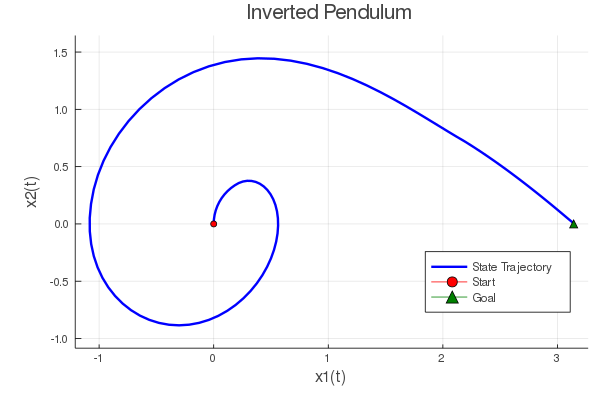
\includegraphics[scale=0.2]{figures/2d_pendulum_spiral}
		\caption{The nominal open-loop trajectory of the $2$-dimensional pendulum.}
		\label{fig:traj 2d pendulum}
	\end{figure}
